\subsection{Integrated anonymous download}
An substantial effort was made to integrated the tunnel community and hidden services community with the MultiChain community.
These communities work together to provide functionality to transfer data anonymously.
The tunnel community reports data transferred between peers and the MultiChain community add these amounts to the chain.
They are already integrated with BarterCast.
The method of integration of BarterCast was used to try to integrated MultiChain aswell.
Setting up the Gumby environment to run all communities took also considerable time.

Experiments were conducted where an 100 MB file is transferred by the actual anonymity communities,
while MultiChain transcribes the transfer amounts in the MultiChain.
The experiment was conducted with 0 hops and 2 hops.
The result of the experiment with 2 hops can be seen in Figure \ref{fig:integrated-anonymous-amounts}.
This shows that MultiChain does track the amount of upload and download for all peers in the network.
The hops roughly download and upload the same amount of their data.
This is what we expected as they just relay the data.
The seeder and leecher respectively only uploads and downloads.

Timeouts can be seen in the plots where the plot hitches and does not grow steadily.
These timeouts occur regularly and should be reduced in the future.
The thresholds of the scheduler of every node is now reached at the same time resulting in a timeout.
Our recommendation is to have these thresholds to be shifted by a small amount randomly for every peer
to prevent them from overlapping.

The result of these experiments show that the integration was not done properly.
There are two problems that were identified using the results of the experiments.

When the experiment is conducted without any hops,
the integration does not report any data transferred between the peers.
As such the scheduler never sees a reason to schedule a signature request.
The whole MultiChain community is never active.
The connection between the seeder and the first hop,
or the downloader, directly is not reported to the scheduler.

Secondly, there is a problem with the amount of data that is reported to be transferred.
Too much data is reported and it is unclear where this data originates from.
The overhead measures twice the actual download size.
The results can be seen in Figure \ref{fig:integrated-anonymous-amounts}.

Integrating MultiChain into the anonymous download communities is difficult,
because those communities do not use the standard classes used by Tribler to send messages.
These are necessary to properly integrate MultiChain and a complicated conversion was necessary.
Our recommendation is to refactor the anonymous download communities to use the standard classes
and to make it more clear in the code where data is sent and where data is received.
Also comments should be added to clarify the code.
Currently there are no comments whatsoever.

\begin{figure}
\centering
\subfigure[Total download amount.]{
\centerline{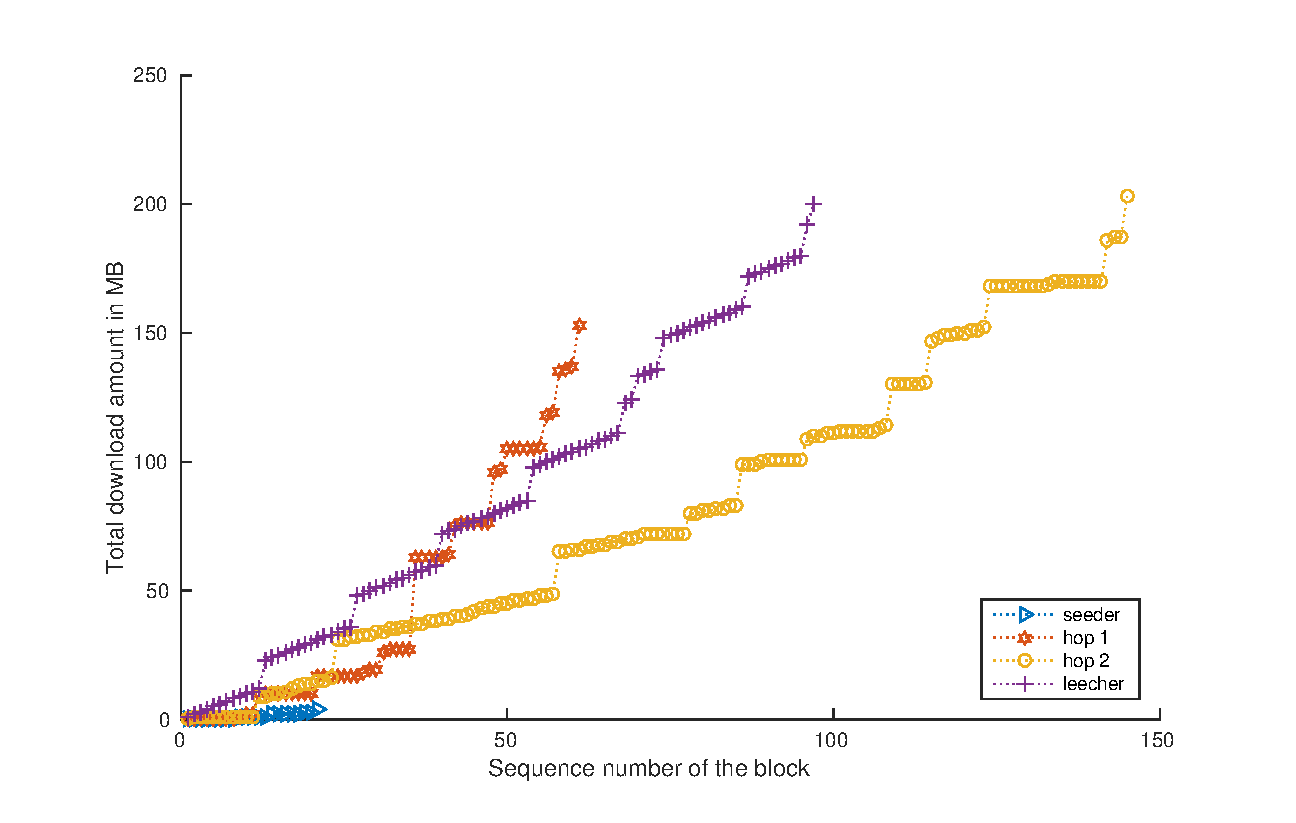
\includegraphics[scale=0.5]{experimentation/anonymous-integrated/integrated-anonymous-down.eps}}
\label{fig:integrated-anonymous-down}
}
\subfigure[Total upload amount.]{
\centerline{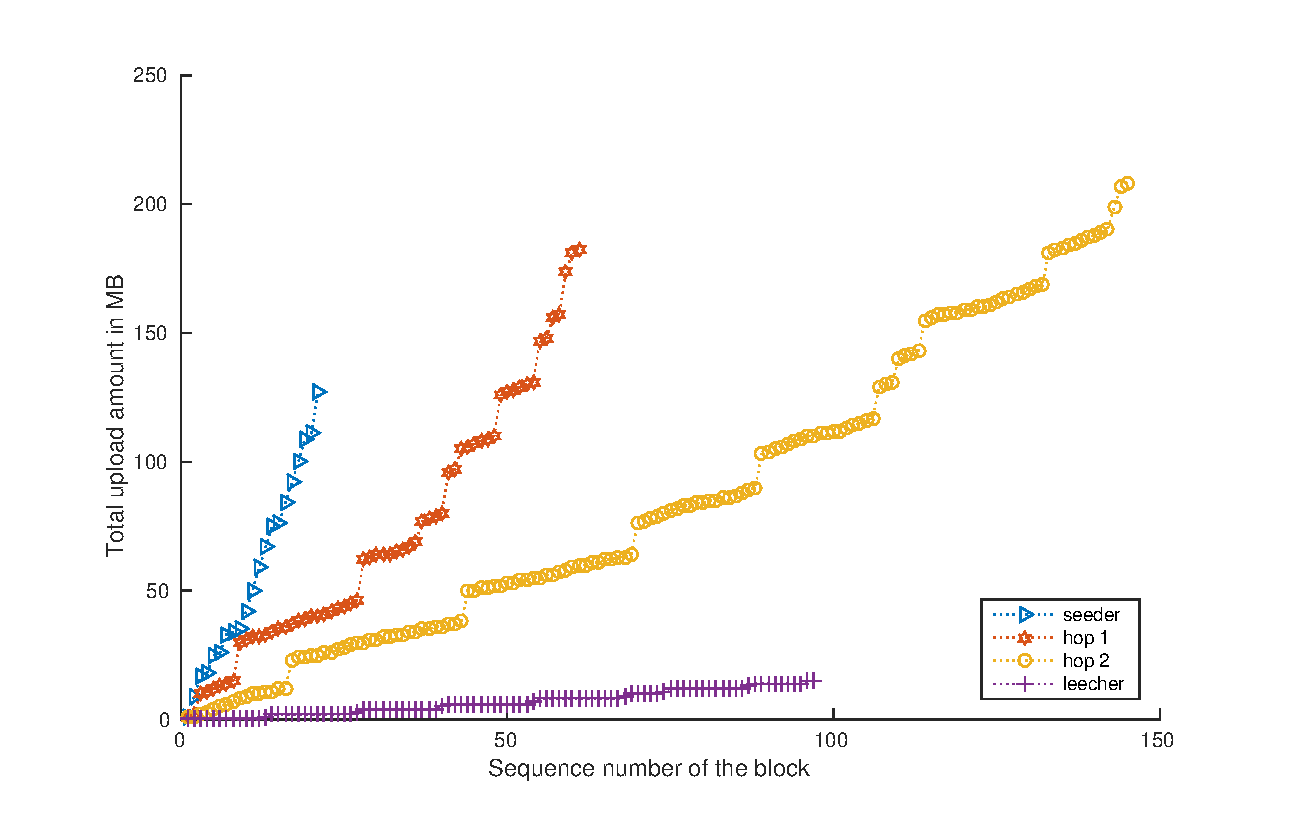
\includegraphics[scale=0.5]{experimentation/anonymous-integrated/integrated-anonymous-up.eps}}
\label{fig:integrated-anonymous-up}
}
\caption{Download and upload amounts during the integrated anonymous download experiment.}
\label{fig:integrated-anonymous-amounts}
\end{figure}